\documentclass[tikz,border=10pt]{standalone}
\begin{document}
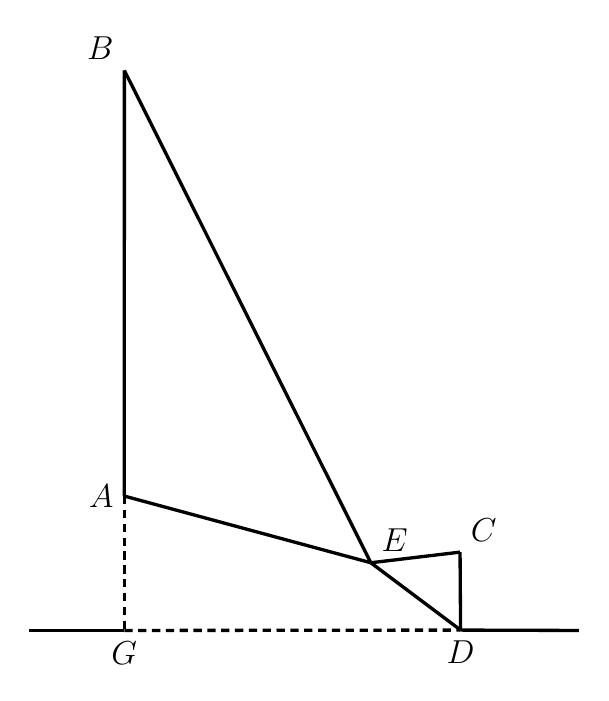
\begin{tikzpicture}[line width=1.2pt, line join=round]
\coordinate (A) at (-2.283,-1.849);
\coordinate (B) at (-2.282,3.556);
\coordinate (C) at (1.981,-2.561);
\coordinate (D) at (1.988,-3.551);
\coordinate (G) at (-2.283,-3.556);



\coordinate (E) at (0.848,-2.696);


\draw (-3.489,-3.556) -- (G);
\draw[dash pattern=on 3pt off 2pt] (G) -- (D);
\draw (D) -- (3.489,-3.556);


\draw (B) -- (A);
\draw[dash pattern=on 3pt off 2pt] (A) -- (G);


\draw (B) -- (E);
\draw (A) -- (E);
\draw (E) -- (D);
\draw (E) -- (C);


\draw (C) -- (D);


\node[above left, font=\fontsize{12}{14.4}\selectfont] at (B) {$B$};
\node[left, font=\fontsize{12}{14.4}\selectfont] at (A) {$A$};
\node[below, font=\fontsize{12}{14.4}\selectfont] at (G) {$G$};
\node[below, font=\fontsize{12}{14.4}\selectfont] at (D) {$D$};
\node[above right, font=\fontsize{12}{14.4}\selectfont] at (E) {$E$};
\node[above right, font=\fontsize{12}{14.4}\selectfont] at (C) {$C$};
\end{tikzpicture}
\end{document}